
\begin{figure}[t]

\centerline{
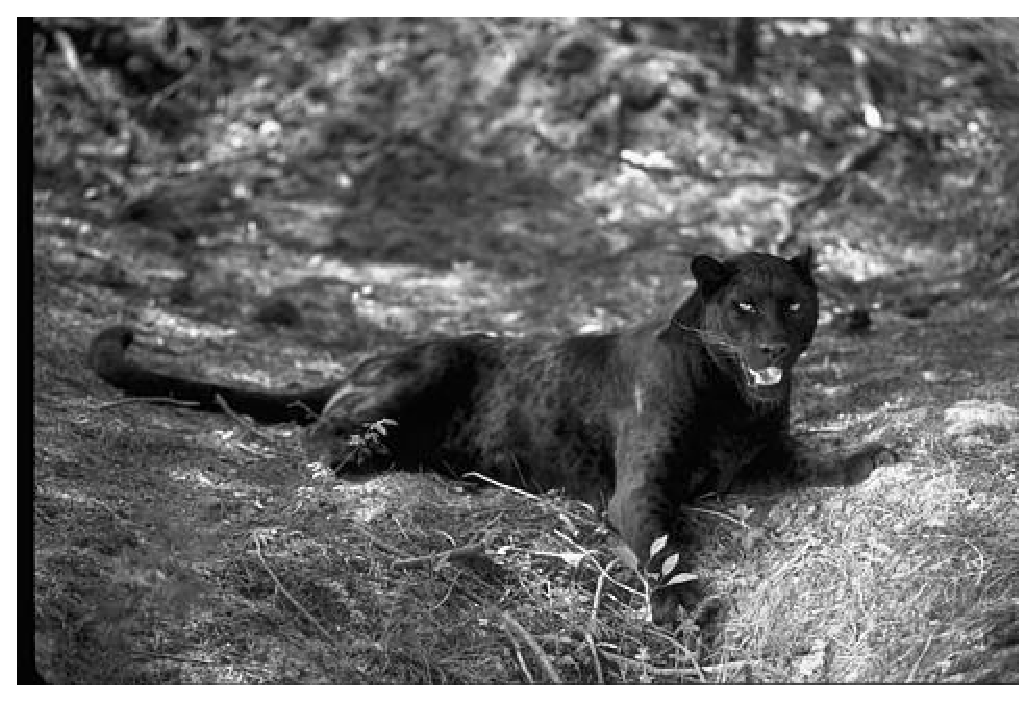
\includegraphics[width=0.3\columnwidth]{cat}
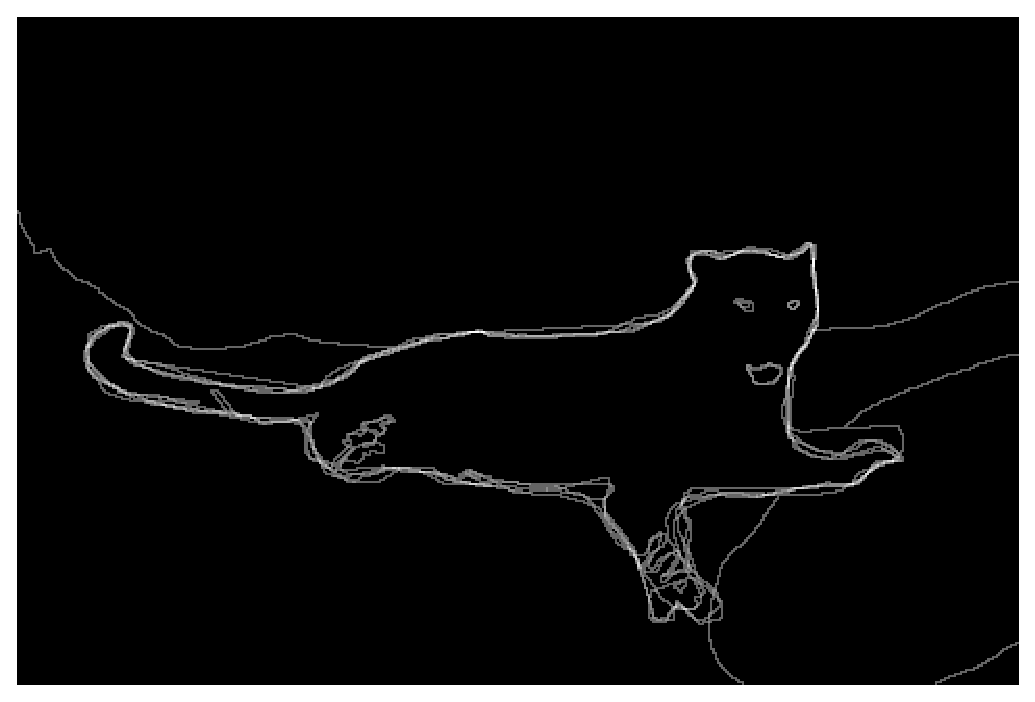
\includegraphics[width=0.3\columnwidth]{cat-human}
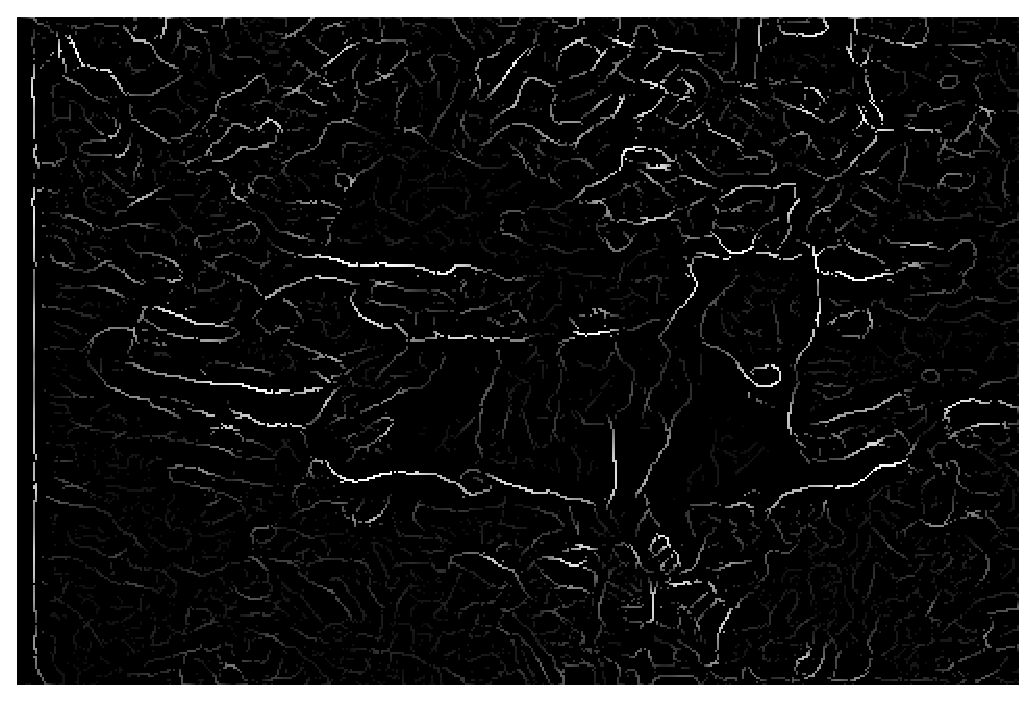
\includegraphics[width=0.3\columnwidth]{cat-machine}
}

\caption[Object segregation is difficult for machines]{
%
\ifcapped
%
An example from \citeasnoun{martin04learning}, to highlight
the difficulties of bottom-up segmentation.
For the image shown on the left, humans see the definite boundaries
shown in white in the middle image.
The best machine segmentation of a set of algorithms gives the
result shown on this right -- a mess.  This seems a very difficult 
scene to segment without having some training at least for the specific 
kinds of materials in the scene.
%
\fi
%
}

\label{fig:segmentation-is-hard}

\end{figure}




The world around us has structure, and to an adult appears to be made
up of more-or-less well-defined objects.  
%
Perceiving the world this way sounds trivial, but from an engineering
perspective, it is heart-breakingly complex.  As Spelke wrote in 1990:

\begin{quote}

... the ability to organize unexpected, cluttered, and
changing arrays into objects is mysterious: so mysterious
that no existing mechanical vision system can accomplish this task
in any general manner.
\cite{spelke90principles}

\end{quote}

\noindent
This is still true today.  This ability 
to assign
boundaries to objects in visually presented scenes 
(called ``object segregation''
in psychology or ``object segmentation'' in engineering) cannot yet be
successfully automated for arbitrary object sets in unconstrained
environments (see Figure~\ref{fig:segmentation-is-hard}).

On the engineering side, there has been some {\em algorithmic} progress; for
example, given local measures of similarity between each neighboring
element of a visual scene, a globally appropriate set of boundaries
can be inferred in efficient and well-founded ways (see for example
\citeasnoun{shi00normalized,felzenszwalb04efficient}).
%
%
Just as importantly, there is also a growing awareness of the
importance of collecting and exploiting empirical {\em knowledge}
about the statistical combinations of materials, shapes, lighting, and
viewpoints that actually occur in our world (see for example
\citeasnoun{martin04learning}).  Of course, such knowledge can only be
captured and used effectively because of algorithmic advances in
machine learning, but the knowledge itself is not specified by an
algorithm.

Empirical, non-algorithmic knowledge of this kind now plays a key role
in machine perception tasks of all sorts.
%
For example, face detection took a step forward with
\citeasnoun{viola04robust}; the success of this work was due both to
algorithmic innovation and better exploitation of knowledge (features
learned from 5000 hand-labelled face examples).
%
The success of automatic speech recognition is successful largely
because of the collection and exploitation of extensive corpuses of
clearly labelled phoneme or phoneme-pair examples that cover well the
domain of utterances to be recognized.
%

These two examples clarify ways ``knowledge'' can play a role in
machine perception.  The bulk of the ``knowledge'' used in
such systems takes the form
of {\em labelled examples} -- examples of input from the sensors (a
vector of numbers), and the corresponding desired output
interpretation (another vector of numbers).  
%
More-or-less general
purpose machine learning algorithms can then approximate the mapping
from sensor input to desired output interpretation based on the
examples (called the {\em training set}), and apply that approximation to novel
situations (called the {\em test set}).  
%
Generally, this approximation will be very poor unless we transform
the sensory input in a manner that highlights properties that the
programmer believes may be relevant.  This transformation is called
{\em preprocessing and feature selection}.
%
There is a great deal of
infrastructure wrapped around the learning system
to break the problem down into tractable parts and
apply the results of learning back to the original
problem.
%
%How good the
%approximation is will depend on a lot of factors.  Researchers try to
%reduce the need for manual feature selection, eliminate the need for
%labels, reduce the number of examples needed, etc.
%
For this paper, we will group all this infrastructure and call it 
the {\bf \em algorithmic skeleton}.
%
%
This set of carefully interlocking algorithms is designed so that,
when fed with appropriate training data, it fleshes out into a
functional system.  Without the algorithmic skeleton, there would be
no way to make sense of the training data, and without the data,
perception would be crude and uninformed.

What, then, is the right algorithmic skeleton for object
segregation?  What set of algorithms, coupled with what kind of
training data, would lead to best performance?  
%
%No-one knows.
%
We review suggestive
work in infant development research and robotics.


%Answering this is not
%easy, and is a potential area for fruitful interaction between infant
%development research and robotics.  We return to this point in the
%conclusions.  But now, we dip into the authors' object segregation
%work on infants and robots, and see how they relate.





\begin{figure}

\centerline{
\includegraphics[width=0.75\columnwidth]{fig-seg}}

\caption[Object segregation is not always well-defined]{
%
\ifcapped
%
Object segregation is not necessarily well-defined.
%
%Image segmentation and object segregation are different.  
%
On the left,
there is a simple scenario, taken from \citeasnoun{needham01object},
showing a rectangle attached to a yellow tube.  Two 
plausible ways to segregate this scene are shown in the middle,
depending on whether the tube and rectangle make up a single 
object.
%
For
comparison, automatically acquired boundaries are shown on the right,
produced using the algorithm in
\citeasnoun{felzenszwalb04efficient}. 
This algorithm does {\em image segmentation},
seeking to produce regions that correspond to whole objects (such as the
 yellow
tube) or at least to object parts (such all the blue rectangle and all
the small white patches on its surface, and various parts of the
background).  Ideally, regions that extend across object boundaries
are avoided.  Image segmentation is less ambitious than object segregation,
and allows context information to be factored in as a higher level
process operating on a region level rather than pixel level.
%
% higher-level processes need only consider merging
%regions (of which there are a relatively small number) rather than
%splitting regions (which requires a return to pixel-level
%considerations).  
%
%
%
%
%
%
\fi
%
}

\label{fig:image-segmentation}

\end{figure}



%In this paper, we
%stick with the term from psychology.  In computer vision, object
%segregation turns out to be a key, but very difficult task, and most
%general-purpose work instead focuses on the (still difficult) task of
%``image segmentation'': grouping regions of similar appearance that
%may correspond to either an object or part of an object.
%
%More on this later.
%

%In psychology, the human ability to divide a scene into a set of
%discrete objects is termed ``object segregation.''  

%In computer vision and robotics, there are algorithms with 
%similar goals.  


%\subsection{Development of segregation skills in infants}
\subsection{Segregation skills in infants}

\label{sect:infant-skills}

%Development of object segregration skills in infants}

%It is clear that human infants learn generic principles for making
%educated guesses about which surfaces belong together as part of the
%same unit and which do not.  
%
By 4 to 5 months of age, infants can
visually parse simple displays like the one in 
Figure~\ref{fig:image-segmentation}
 into units, based on something like 
a subset of static
Gestalt principles~--
%, probably some subset of these
 see for example \citeasnoun{needham98infants,needham00improvements}.
%
%with partly occluded objects (JOHNSON)). 
%
%Similar results have been obtained by researchers using partly
%occluded objects (Johnson).
%
Initial studies indicated that infants use a collection of
features to parse the displays \cite{needham98infants,needham97object,needham98effects}; subsequent studies suggested that object shape is the key
feature that young infants use to identify boundaries between adjacent
objects \cite{needham99role}.
%
%Ongoing work aims at elucidating the role of different features
%at different ages.
%
Compared to adult judgements,
%
we would expect such strategies to lead to many incorrect parsings, 
but they will
also provide reasonable best guess interpretations of uniform objects
in complex displays.  



Infants do not come prepared from birth to segregate objects into 
units that match adult judgement.
%
%adults would consider meaningful.  
%
It appears that infants learn over time how object
features can be used to predict object boundaries.  More than twenty
years ago, \citeasnoun{kellman83perception} suggested that infants may be born
with knowledge about solid, three-dimensional objects and that this
knowledge could help them interpret portions of a moving object as
connected to other portions that were moving in unison.  This
assertion was put to the test by Slater and his colleagues 
\cite{slater90newborn}, a test that resulted in a new conception of
the neonate's visual world.  Rather than interpreting common motion as
a cue to object unity, neonates appeared to interpret the visible portions of a
partly occluded object as clearly separate from each other, even when
undergoing common motion.  This finding was important because it
revealed one way in which learning likely changes how infants
interpret their visual world.


Although segregating adjacent objects present a very similar kind of
perceptual problem (``are these surfaces connected or not''), the
critical components of success might be quite different.  Early work
with adjacent objects indicated that at 3 months of age, infants tend
to group all touching surfaces into a single unit
\cite{kestenbaum87perception}.  Subsequent experiments have revealed
that soon after this point in development, infants begin to analyze
the perceptual differences between adjacent surfaces and segregate
surfaces with different features (but not those with similar features)
into separate units (Needham 2000).
%
\ifverbose
Although infants can use the boundary seam between
two objects as a source of information about the likely separation
between them (Kaufman \& Needham, submitted), other work comparing
boundary-occluded and fully visible versions of the same displays
suggests that boundary information is not the only information infants
use to parse the objects in a display (Needham, 1998).  
\fi
%
Still later,
8.5 month old infants have been shown to also use information about specific
objects or classes of objects to guide their judgement (Needham,
Cantlon, \& Ormsby, 2005).


%%\subsection{Development of segregation skills in infants}

It might be that extensive amounts of experience are required to
`train up' this system.  However, it might also be that infants learn
on the basis of relatively few exposures to key events (Baillargeon,
1999).  This possibility was investigated within the context of object
segregation by asking how infants' parsing of a display would be
altered by a brief prior exposure to one of the objects in the test
display.


In this paradigm, a test display was used that was ambiguous to
4.5-month-old infants who had no prior experience with the display.
Prior experience was then given that would help disambiguate the display
for infants.  This experience consisted of a brief prior exposure
(visual only) to a portion of the test display.  If infants used this
prior experience to help them parse the test display, they should see
the display as two separate objects and look reliably longer when they
moved as a whole than when they move separately.  Alternately, if the
prior experience was ineffective in altering infants'
interpretation of the display, they should look about equally at the
display, just as the infants in the initial study with no particular
prior experience did \cite{needham98effects}.  Prior experiences
with either portion of the test display were effective in facilitating
infants' parsing of the test display.  

%
%The closest to ``key events'' are the examples presented in training
%data, labelled by hand.



\subsection{Segregation skills in robots}

%%\subsection{Development of object segregration skills in robots}


This idea that {\em exposure to key events} could influence
segregation is intuitive, and evidently operative in infants.  Yet it
is not generally studied or used in mechanical systems for object
segregation.  In this section, we attempt to reformulate robotics
work by the authors in these terms.

For object segregation in robotics, we will interpret ``key events''
as moments in the robot's experience where the true boundary of an
object can be reliably inferred.  They offer an opportunity to
determine {\em correlates} of the boundary that can be detected
outside of the limited context of the key events themselves.  Thus,
with an appropriate algorithmic skeleton, information learned during
key events can be applied more broadly.

Key events in infants include seeing an object in isolation
or seeing objects in relative motion.  In the authors' work,
 algorithmic skeletons have been developed for exploiting
constrained analogues of these situations.

%
In \citeasnoun{natale05exploring}, a very simple key event is used to
learn about objects~-- {\em holding an object up to the face}.
%
The robot can be
 handed an object or happen to grasp it, 
and will then hold it up close to its cameras.
This gives a good view of its surface features, allowing the robot to
do some learning and later correctly segregate the object
out from the background  visually even when out of its
grasp (see Figure~\ref{fig:robot}).
%
%Doing all this requires another algorithmic skeleton of the same 
%structure as the ``poking'' case (though of course with different 
%algorithms to achieve each step).
%
This is similar an isolated presentation of an object, as in
Needham's experiments.  In real
environments, true isolation is very unlikely, and actively
moving an object so that it dominates the scene can be
beneficial.



%The key event for infants in the experiments by Needham was 
%relative motion~-- the separate identify of two objects was
%revealed if they moved independently.  
%
%Motion relative to 
%a fixed background is a cue used constantly in computer vision.
%


In \citeasnoun{fitzpatrick03grounding}, the ``key event'' used is {\em
hitting an object with the hand/arm}.  This is a constrained form of
relative object motion.  In the real world, all sorts of strange
motions happen which can be hard to parse, so it is simpler at least
to begin with to focus on situations the robot can initiate and at
least partially control.
%
%This is a much narrower kind of motion than that considered by
%Needham and colleagues.  Ultimately, robots should be equally
%flexible, but for now the automatic interpretation of general motion of
%objects is of disappointing quality.
%
Motion caused by body impact has some technical advantages; the
impactor (the arm) is modelled and can be tracked, and since the moment 
and place of
impact can be detected quite precisely, unrelated motion in the scene
can be largely filtered out.

The {\em algorithmic skeleton} in \cite{fitzpatrick03grounding}
processes views of the arm moving, detects impacts, and
outputs boundary estimates of whatever the arm collides with based on
motion.  These boundaries, and what they contain, are used as training
data for another algorithm, whose purpose is to estimate boundaries
from visual appearance when motion information is not available.
%
%
See \citeasnoun{fitzpatrick03object} for technical details.
As a basic overview, the classes of algorithms involved are these:


%As a taste of what
%is learned in Figure~\ref{fig:robot}, a large collection of (probabilistic)
%rules of the following nature are learned: if there are two edges at a
%specific angle to each other, and of specific relative scales, and
%between them lies a surface of an approximate color, then there {\em
%might} be a specific object at a specific relative location, angle,
%and scale.  These rules are used in practice to scan an image, find
%locations that many rules suggest might hold a specific object, and
%work back to figure out which edges in the image are likely to form
%the silhoette of that object.

%The {\em algorithmic skeleton} here is: 

\begin{enumerate} \pflist

\item {\em Behavior system}: an algorithm that drives the robot's
behavior, so that it is likely to hit things.  This system has a 
broader agenda than just this specific outcome:

\item {\em Key event detection}: an algorithm that detects the key event of
when the arm/hand hits an object.

\item {\em Training data extraction}: an algorithm that, within a key event,
extracts boundary information from object motion caused by hitting.

\item {\em Machine learning}: an algorithm that discovers features
predictive of boundaries that can be extracted in other situations
without motion (in this case edge and color combinations).

\item {\em Application of learning}: an algorithm that actually uses
those features to predict boundaries.  This must be integrated with
the very first algorithm, to influence the robot's behavior in useful
ways.  In terms of observable behavior, the robot's ability to attend
and fixate specific objects increases, since they become segregated from
the background.

\end{enumerate}

\noindent
This skeleton gets fleshed out through learning, once the
robot actually starts hitting objects and extracting specific features
predictive of the boundaries of specific objects.  
%
A set of different algorithms performing analogous roles are used
for the \citeasnoun{natale05exploring} example.
%
%
At the algorithmic level, the technical concerns 
in either
case are hard to relate to
infant development, although in some cases there are correspondences.
%
But at the skeletal level, the concerns are coming closer to those of
infant development.

%The point this paper wishes to make is at the level of the {\em
%algorithmic skeleton}, organized around exploiting {\em key events}
%for improving or at least adapting perceptual skills, there is the
%potential for mutual inspiration and relevance.
%
%Right now, there is a disconnect between the few key events used in
%robotics and the many key events investigated in infant development.
%If the robotics community paid more attention to infant development,
%then more of these key events would be exploited.  The events
%that get exploited earlier and most successfully are thereby
%demonstrated to be truly workable.  Failure to exploit them
%could mean lack of attention, or that 
%they are more complex than they might appear.


%The details of these algorithms are not inspired by, or likely to 
%be relevant to, infant development.  But at the strategic level,
%there is inspiration and potential relevance.  To improve
%the robotic system, we need to identify more key events, and
%wrestle with ....

%
%ARSENIO (2005).


\ifverbose
%
In \citeasnoun{fitzpatrick03grounding}, used
a very specific condition (objects being hit by
people or the robot itself) to extract good
motion-based object boundaries; surface features
of the object could then be used to segregate that
object out in static presentations \cite{fitzpatrick03object}.
\citeasnoun{arsenio05exploiting} used rhythmic motion
of objects to segment their boundaries both in
visually and acoustically.
%
Arsenio (2005) developed a set of techniques for acquiring all
sorts of segmentations.  Some methods work for small, grasp-size
objects, others work for large background objects like walls or
tables.
\fi


\begin{figure}[t]

\centerline{
%%
\includegraphics[width=0.75\columnwidth]{fig-robot}
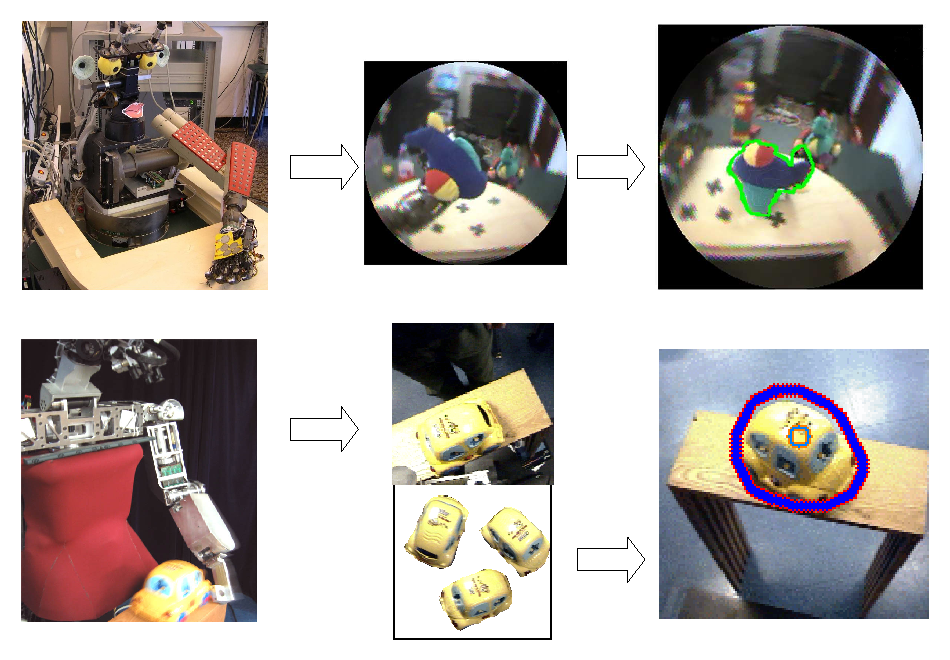
\includegraphics[width=0.75\columnwidth]{fig-robots}
}

\caption[Exploitation of key moments in robotics]{
%
\ifcapped
%
The upper row shows object segregation by the robot ``Babybot'' 
based on prior experience.  
%The holding an object up to 
%Object segregation based on specific object experience.  
%
%Manipulation is another opportunity to perform object segregation. In
The robot explores the visual appearances of an object that
it has grasped; the information collected in this way is used later on to
segment the object \cite{natale05exploring}. 
%
%The exploration in this
%5case is facilitated by a pre-acquired body-schema that allows the
%robot to maintain the fixation of the hand. 
%
Left: the robot.
%, the
%robotic platform used for this experiment. 
Middle: the robot's view when holding up an object.
Right: later segmentation of the object.
%
% (consider moving this figure
%in the segregation-robotics section).
%
The lower row shows the robot ``Cog''
detecting object boundaries experimentally by
poking \cite{fitzpatrick03object}.
%
During object motion, it finds features of the object that contrast with other
objects, and that are stable with respect to certain geometric
transformations.  These features are then used to jointly detect
and segment the object in future views.  Left: the robot.
Middle: segmentations of a poked object.
Right: later segmentation of the object on a
similarly-colored table. 
%%
%%
%%
%
%
\fi
%
}

\label{fig:robot}

\end{figure}





\subsection{Specificity of knowledge gained from experience}


%To learn from experience requires generalization.
%
In the robotic learning examples in 
the previous section \cite{fitzpatrick03object,natale05exploring},
information learned by the robot is intended to be specific to one particular
object.  The specificity could be varied algorithmically,
by adding or removing parts of a feature's ``identity''.
Too much specificity, and the feature will not be recognized
in another context.  Too little, and it will be ``hallucinated''
everywhere.
%
%
%How could such categories be formed?
%

We return to 
Needham's experiments, which probed the question of
generalization in the same
experimental scenario described in Section~\ref{sect:infant-skills}.

When changes were introduced between the object seen during
familiarization and that seen as part of the test display, an
unexpected pattern emerged.  Nearly any change in the object's
features introduced between familiarization and test prevented infants
from benefiting from this prior experience.  So, even when infants
saw a blue box with yellow squares prior to testing, and the box used
in testing had white squares but was otherwise identical, they did not
apply this prior experience to the parsing of the test display.
However, infants did benefit from the prior exposure when it was not
in the features of the object but rather in its orientation 
 \cite{needham01object}.  
A change in the orientation of the box from horizontally to
vertically oriented led to the facilitation in parsing seen in some
prior experiments.  Thus, infants even as young as 4.5- to 5-months of
age know that to probe whether they have seen an object before, they
must attend to the object's features rather than its spatial
orientation \cite{needham01object}.

These results also support two additional conclusions.  First,
infants' object representations include detailed information
about the object's features.  Because infants'
application of their prior experience to the parsing of the test
display was so dependent on something close to an exact match between
the features, one much conclude that a highly detailed representation
is formed on the initial exposure and maintained during the
inter-trial-interval.  Because these features are remembered and used
in the absence of the initial item and in the presence of a different
item, this is strong evidence for infants' representational
abilities.  Secondly, 4.5-month-old infants are conservative
generalizers -- they do not extend information from one object to
another very readily.  But would they extend information from a {\bf group}
of objects to a new object that is a member of that group?


%There is no notion of object category.
%
%In this respect, Needham's results on generalizations are
%very interesting, in possibly pointing a way forward.


\subsection{Generalization of of knowledge gained from experience}

This question was investigated by \citeasnoun{needham05infants}
in a study using the same test display and a similar procedure as in
\citeasnoun{needham01object}.  Infants were given prior experiences with collections
of objects, no one of which was an effective cue to the composition of
the test display when seen prior to testing.  A set of three similar
objects seen simultaneously prior to test did facilitate 4.5-month-old
infants segregation of the test display.  But no subset of these three
objects seen prior to testing facilitated infants' segregation of the
test display.  Also, not just any three objects functioned in this way
-- sets that had no variation within them or that were too different
from the relevant test item provided no facilitation.  Thus,
experience with multiple objects that are varied but that are similar
to the target item is important to infants' transfer of their
experience to the target display.


This finding 
with artifical objects was tested in a more natural setting
%
%was brought into the ``real'' world 
%
by investigating
infants' parsing of a test display consisting of a novel key
ring (Needham et al., submitted).  
%
According to a strict
application of organizational principles using object features, the
display should be seen as composed of (at least) two separate
objects -- the keys on one side of the screen and the separate
ring on the other side.  However, to the extent that infants recognize
the display as a member of a familiar category -- key
rings -- they should group the keys and ring into a single unit
that should move as a whole.  The findings indicate that by 8.5 months
of age, infants parse the display into a single unit, expecting the
keys and ring to move together.  Younger infants do not see the
display as a single unit, and instead parse the keys and ring into
separate units.  Infants of both ages parsed an altered display, in
which the identifiable portions of the key ring were hidden by
patterned covers, as composed of two separate units.  Together, these
findings provide evidence that the studies of controlled prior
exposure described in the previous section are consistent with the
process as it occurs under natural circumstances.  Infants'
ordinary experiences present them with multiple similar exemplars of
key rings, and these exposures build a representation that can then be
applied to novel (and yet similar) instances of the key ring category,
altering the interpretation that would come from feature-based
principles alone.


\ifverbose
Supporting a differentiation view of the development of
generalization, Bahrick's findings suggest that young (i.e.,
2-month-old) infants are more likely to generalize farther from the
specific experiences they received than infants just a few months
older (get citation).  This finding suggests that experience might
serve to initially narrow and then extend the range of stimuli over
which young children will generalize.
\fi

These results from infant development suggest a path for
robotics to follow.  There is currently no serious robotics
work to point to in this area, despite its importance.
Robotics work in this area could potentially aid infant
psychologists since there is a strong theoretical framework
in machine learning for issues of generalization.



